\documentclass[12pt,french,titlepage]{article}
\usepackage[utf8]{inputenc}
\usepackage{geometry}
\usepackage{amsfonts}
\usepackage{float}
\usepackage{graphicx}
\usepackage{hyperref}
\hypersetup{colorlinks,urlcolor=blue}
\geometry{
 a4paper,
 left=25mm,
 right=25mm,
 top=25mm,
 bottom=25mm
 }
\title{\textbf{Game of Thrones} \\ House of D2SI}
\date{\vspace{-35ex}}
\begin{document}
\maketitle

\section{Context}
Aemon the Castle Black's maester is a close advisor of Jeor Mormont, the Lord Commander. He is also the Castle Black's library director. This library has hundreds of thousands of books and some of them are so rare you can not even find them in the Citadel. 
\\\\
Searching information in this huge books collection is getting more and more challenging for Aemon as the years pass. He decided to ask Sam, his favorite trainee for some help to find a way to easily \textbf{search information in documents from keywords}. Then Sam asked his friend Jon Snow who always liked information search and data engineering.
\\\\
Jon Snow decided to use vector representation of documents. Search engines use different kind of document representations and one of them is the vector representation. It gives the ability to directly use mathematical tools such as distance, similarity and dimension reduction.
\\\\
Our challenge is not about those mathematical tools but is about building an \textbf{inverted index} of the documents to speed up calculations. Indeed those calculations are often based on dot products that consume a lot of CPU and memory. Having an inverted index simplifies those dot products.
\\
We want to write an efficient implementation to build an inverted index of a large collection of documents.

\section{Algorithm}
\subsection{Documents}
We have a collection of N documents. In our case we have one file per document and the name of a file is simply the indice of the document as shown on the figure \ref{fig:documents}.
\begin{figure}[H]
    \centering
    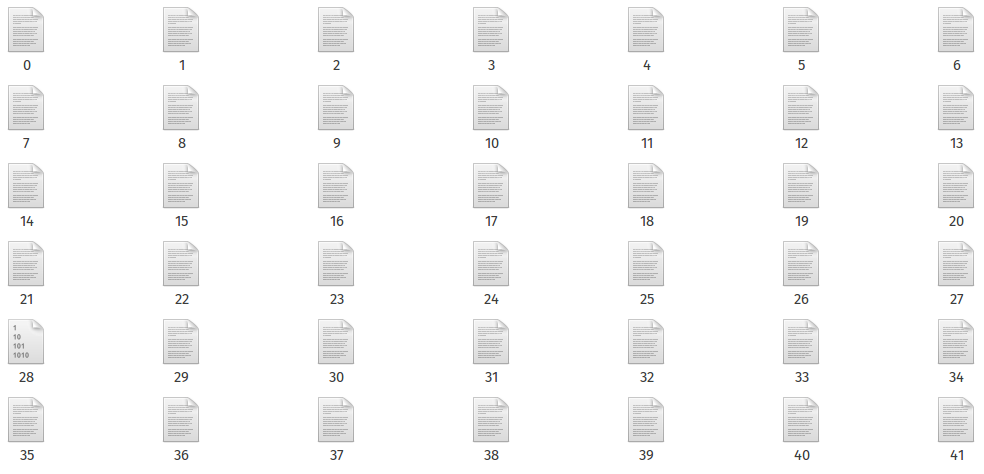
\includegraphics[scale=0.45]{images/dataset}
    \caption{Document collection}
    \label{fig:documents}
\end{figure}
\subsection{Dictionnary}
We want a dictionnary that matches every word from the documents with a unique id. See the figure \ref{fig:dictionnary} for a sample.
\begin{figure}[H]
    \centering
    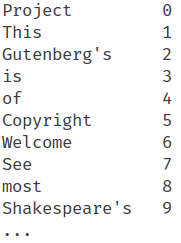
\includegraphics[scale=0.75]{images/dictionnary}
    \caption{Dictionnary example}
    \label{fig:dictionnary}
\end{figure}
\subsubsection{Inverted index}
Using both the dataset and the dictionnary we can build an inverted index that gives, for every word, the list of documents it appears in. See the figure \ref{fig:inverted_index}.
\begin{figure}[H]
    \centering
    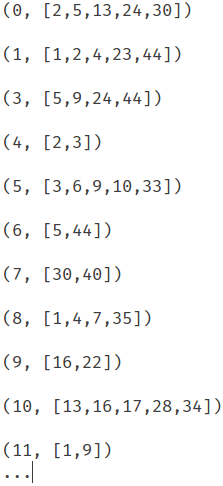
\includegraphics[scale=0.65]{images/inverted_index}
    \caption{Inverted index example}
    \label{fig:inverted_index}
\end{figure}
We want a solution that works on a massive dataset. Our algorithm has to be able to run on a distributed system so we are not limited by the amount of storage, memory and CPU of a single machine. 
\\\\
These are the 4 steps of the algorithm. See also the figure \ref{fig:algorithm_steps}.
\begin{enumerate}
    \item Read the documents and collect every pair (wordID, docID)
    \item Sort those pairs by wordID and by docID
    \item For every wordID, group the pairs so you have its list of documents
    \item Merge the intermediate results to get the final inverted index
\end{enumerate}
\begin{figure}[H]
    \centering
    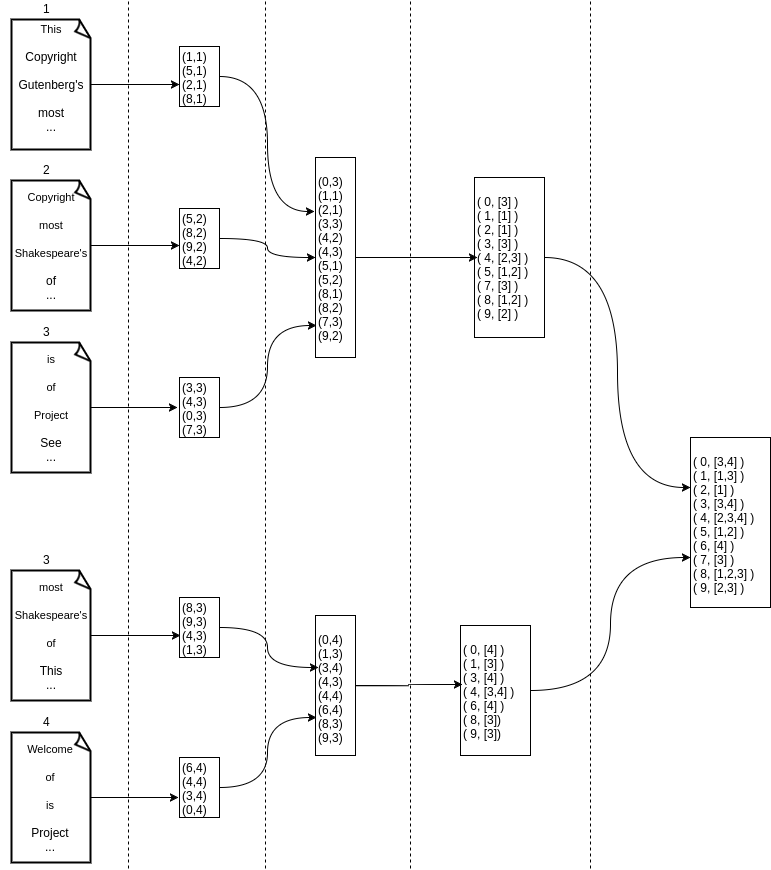
\includegraphics[scale=0.6]{images/algorithm}
    \caption{Algorithm steps}
    \label{fig:algorithm_steps}
\end{figure}
\textbf{NB:} the index must be sorted by the words ids, and for every word id the matching list must be sorted by the documents ids.
\\
Associated algorithm: \href{https://nlp.stanford.edu/IR-book/html/htmledition/blocked-sort-based-indexing-1.html}{\underline{Blocked sort-based indexing}}

\section{Questions}
You will find the dataset of documents in the \textit{dataset} folder of the repository.
\paragraph{1.} Implement a job to build the dictionnary. Every line of the output file will be the word and its id. In the documents of the given dataset the words are separated by one or multiple spaces.
\paragraph{2.} Implement one or multiple jobs to build the inverted index.
\\\\
You may use Hadoop or Spark for those jobs, and the language you prefer.
\end{document}
